\chapter{Instructions} \label{inst}

\section{How to use LaTeX}

Here is some text.\footnote{Here is the footnote.} \cam{comment}\jim{reply}\lucy{counter-reply}\lucy{I'm pink...}This is a sentence that has a footnote at the end of it. To put in a citation, you need the citation key in the bibliography.\footcites{oecd2015,goss2016} You can even put page numbers in the citation.\footcite[][19--21]{wu2010} If, for whatever reason, you want the citation to appear in the text, you do it like this: \textcite{marks2015}.

To start a new paragraph, leave a blank line between. To cross-reference a figure, use \Cref{fig:PoP} or \Vref{fig:57} (note that the figures below in the text below have been labelled). The advantage of using Vref is that the output will tell the reader where to find the figure.

\begin{figure}[p] 
 \caption{The relationship between NAPLAN scale scores and year level is not linear for the median student}
 \units{NAPLAN scale score of median student in each year level, Australia}
 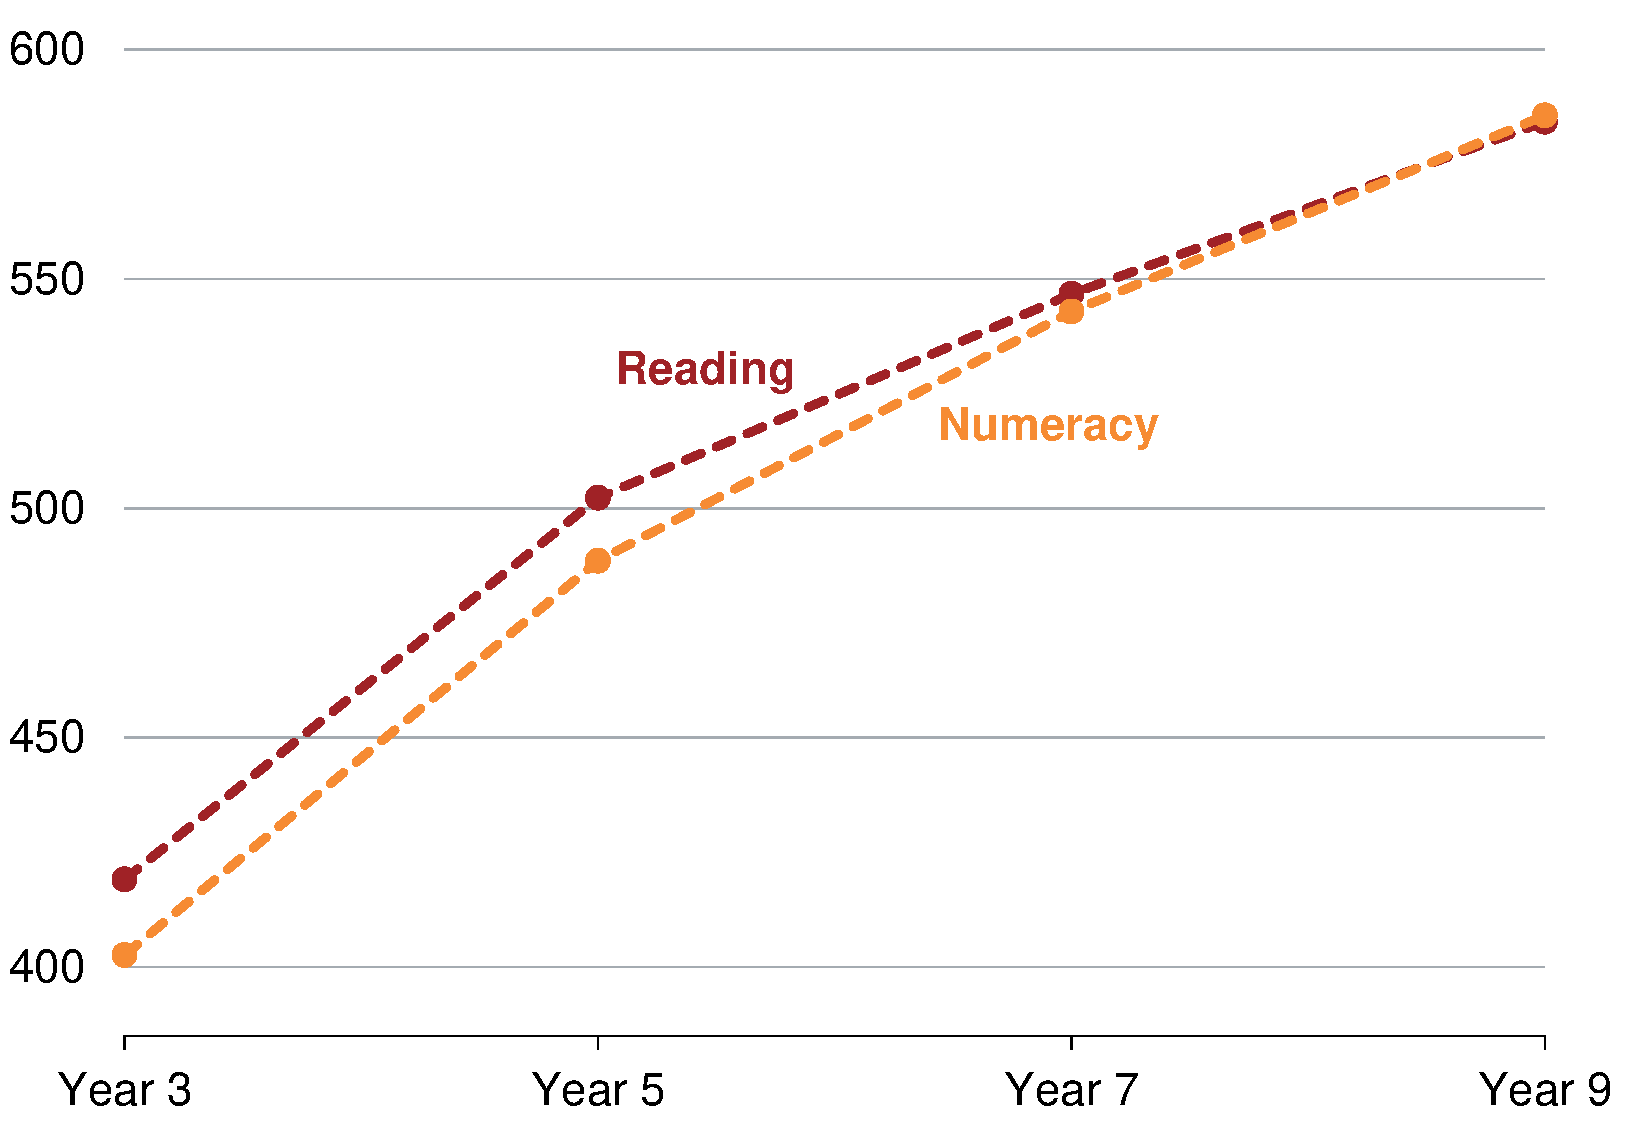
\includegraphics[page=1]{atlas/PoP.pdf}\label{fig:PoP}
\notes{Based on 2014 and 2012 median scores.}

\source{Grattan analysis of \textcite{acara2014}.}
\end{figure}
\begin{figure}[p]
 \caption{Data from Years 5 and 7 students provides a reasonable approximation for other year levels}
 \units{Estimated median NAPLAN scale score, Australia}
 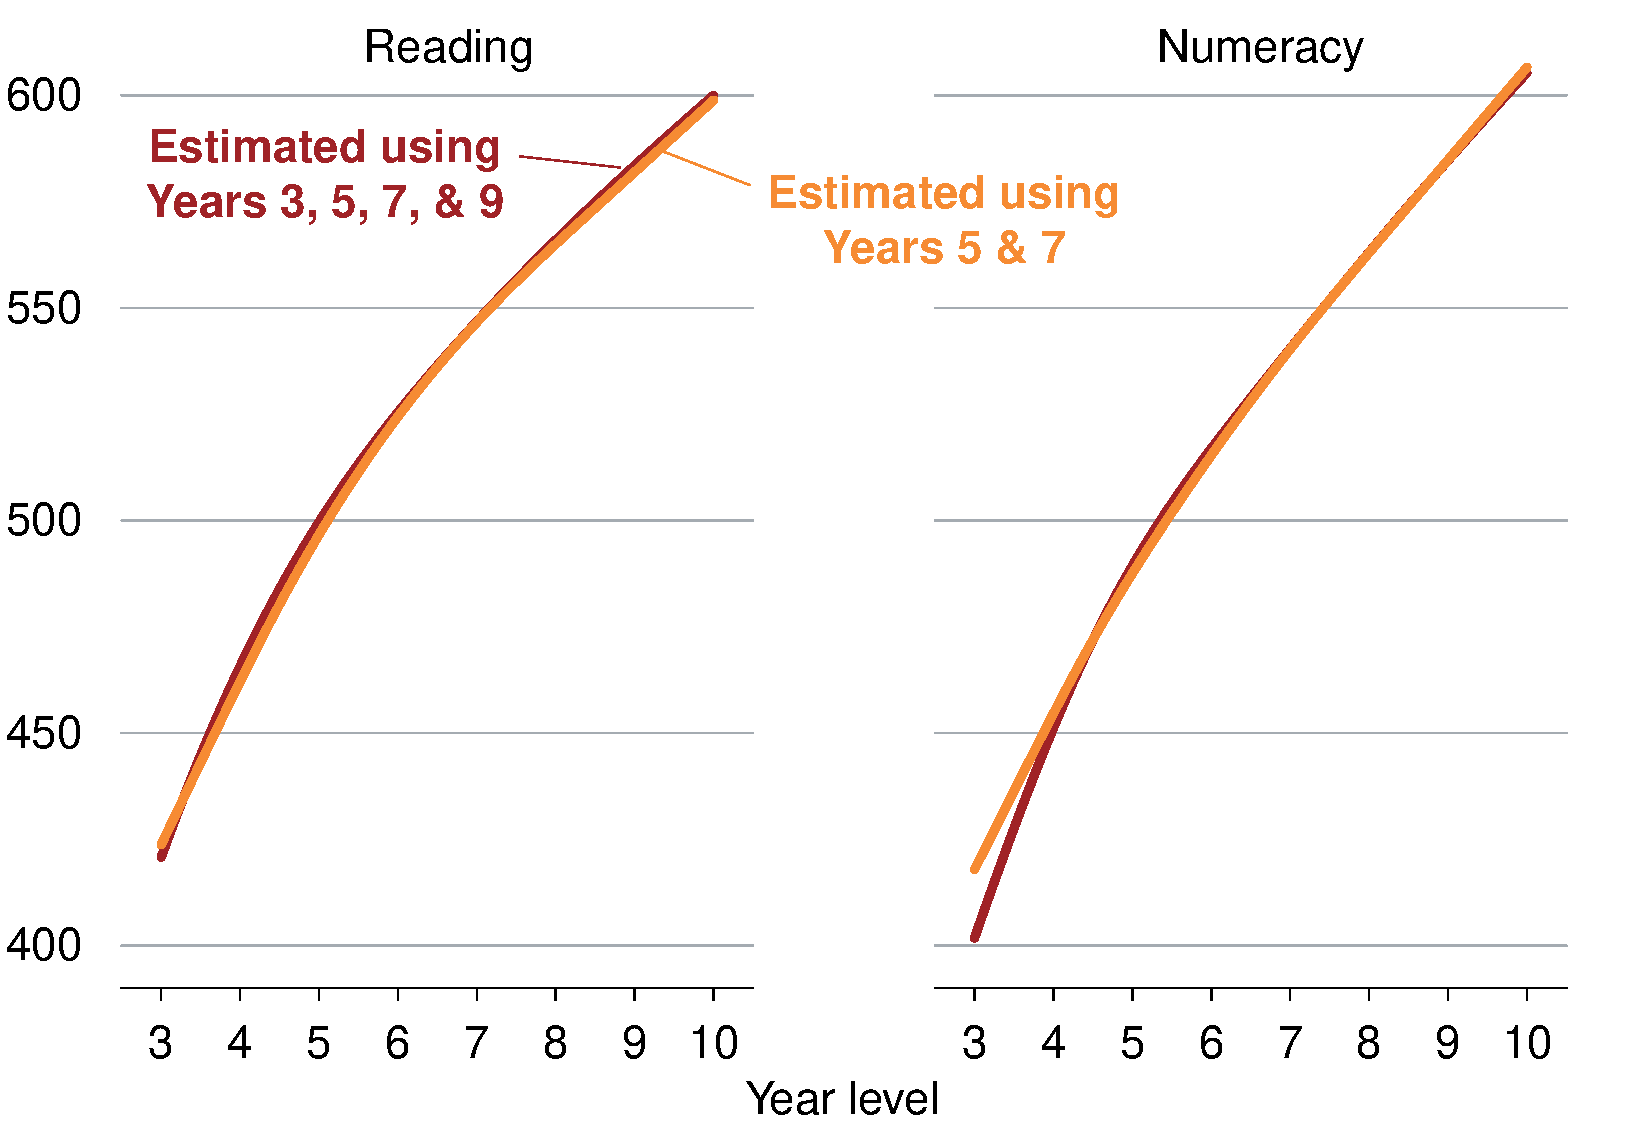
\includegraphics[page=1]{atlas/five_seven.pdf}\label{fig:57}
\source{Grattan analysis of \textcite{acara2014}.}
\end{figure}


Note that charts are saved as PDF files under `atlas'. These can either be saved as individual files, or as a single chart pack (in which case, just refer to the page number of the relevant chart). 

LaTeX places figures at the top of the next available column by default, and does not include text below the chart. This can be overridden, but best practice is to leave the charts in their default position until publication.

Boxes work in a similar way -- they usually appear in their own column (or across two columns). % note that the n-dash uses two hyphens
A single-column box is called a `smallbox', which a two-column box is a `bigbox'. Here are cross-references to \Vref{box:example,box:large_example}.

\begin{smallbox}{Special characters in LaTeX}{box:example}

Some characters have a special meaning in LaTeX. For example, the percentage sign indicates a comment, the dollars sign is used to specify equations, and backslash preceeds commands. If you wish to put special characters in the text, use the following:

Percentage: \%

Dollars sign: \$

Hash key: \#

Curly braces: \{ and \}

Ampersand: \&

Underscore: \_

Tilde: \~{}

Up-arrow: \^{}

Backslash: \textbackslash

Note also the following:

Hyphen: -

N-dash: --

M-dash: ---

Begin quote: ` or ``

End quote: ' or ''

\end{smallbox}

\begin{bigbox}{Title of big box}{box:large_example}

ACARA implicitly acknowledge the non-linear path of progress in the way that results are reported against \textit{NAPLAN proficiency bands}. There are ten proficiency bands spanning \mbox{Year 3} to \mbox{Year 9}, with equally-spaced cut-points along the NAPLAN scale.\footnote{With the exception of Band 1 and Band 10, each band spans 52 NAPLAN scale points.} These bands are used to define the National Minimum Standards. But because student skill level does not increase linearly over time, the National Minimum Standard increases by two bands between Years 3 and 5, but by only one band between Years 5 and 7 and between Years 7 and 9.\footnote{The National Minimum Standard is Band 2 for \mbox{Year 3}, Band 4 for \mbox{Year 5}, Band 5 for \mbox{Year 7}, and Band 6 for \mbox{Year 9}.} If there was reason to believe that the path of progress should be linear, then the change in the National Minimum Standards between each year level should be consistent.

Six proficiency bands are reported for each year level. For a student to remain in the same \textit{relative} proficiency band, they must move up two bands between Years 3 and 5, then one band between Years 5 and 7, and another band between Years 7 and 9. But students who remain in the same relative band have not necessarily been progressing at the same rate.

\Vref{fig:NPB} provides an example of this -- Student~A moves from Band 4 in \mbox{Year 3} to Band 6 in \mbox{Year 5}, staying two bands above the national minimum standard. Student~B performs consistently in the national minimum standard band, moving from Band 4 in \mbox{Year 5} to Band 6 in \mbox{Year 9}. Both students remain in the same relative proficiency band, which suggests they are learning at the
\begin{figure}[H] % placing figures inside boxes is a little tricky - you have to choose exactly where in the text to place it (if you rely on LaTeX to place the figure, it will choose to place it out of the box). In this example, the figure is placed in the middle of a sentence so that the box is balanced. 

 \boxfigurecaption{The level of growth required to remain in the same relative proficiency band changes with year level}
 \units{NAPLAN proficiency band}
 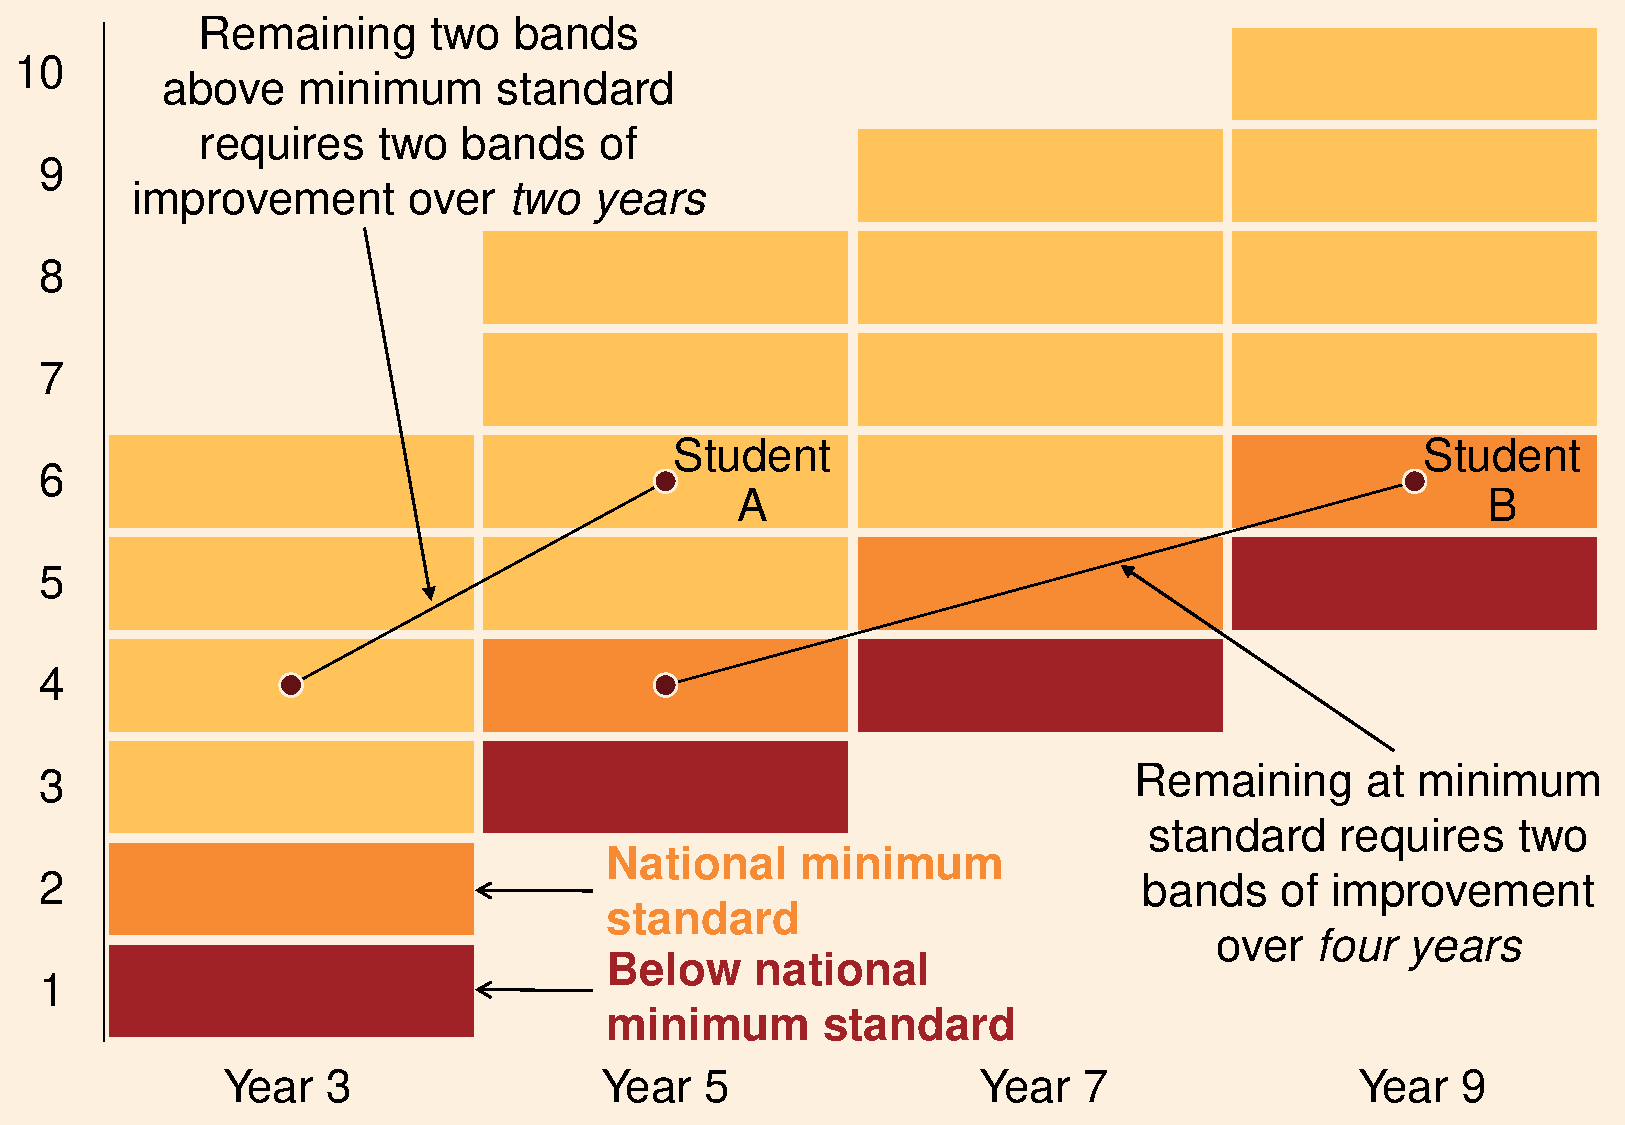
\includegraphics[page=1]{atlas/NPB.pdf}\label{fig:NPB}

\source{\textcite{acara2015a}.}
\end{figure}
\vspace{-10pt}
 same rate. Yet Student~A makes the same gain over two years as Student~B does over four. This suggests that the non-linear scale of proficiency bands does not consistently account for the non-linear path of progress for students at different skill levels.\footnote{The analysis in this report does not use NAPLAN proficiency bands to assess student progress.}

\end{bigbox}

\subsection{Dynamic reporting}

An advantage of \LaTeX{} is that the report can dynamically adapt when key things change. For example, the title of the report may change before publication, and a headline figure may need updating when new data are available.

To refer to the title of the report, use \fulltitle{} (includes the subtitle), or \mytitle{} (does not include the subtitle). That way, if the title of the report changes, it is not necessary to change it every time it is referenced. The curly braces ensure that there will be a space after the title.

If you want to use a headline figure that can be changed, it is first necessary to define it. Use:

%\def\headline{\$10~billion} (as a general rule, it is best to define this in the preamble).

Then, you can refer to it using \headline{}. Note that the `~' sign represents a hard space, ensuring that \headline{} does not appear over two lines.